% Supplementary Material
% Simulator validations and response-metric robustness analyses
% supporting the main text.
% Target journal: Journal of Applied Physics (AIP; REVTeX 4-2, jap substyle).
%
% Build (same directory as ref.bib):
%   pdflatex supplementary
%   bibtex   supplementary
%   pdflatex supplementary  (x2)

%% reprint+onecolumn: `onecolumn` alone leaves REVTeX in its preprint layout
%% (12 pt, double-spaced, separate title page). `reprint` selects the compact
%% single-spaced journal layout and `onecolumn` overrides its column count.
\documentclass[aip,jap,reprint,onecolumn,superscriptaddress,longbibliography]{revtex4-2}
\pdfoutput=1
\usepackage[T1]{fontenc}
\usepackage{amsmath,amssymb,graphicx,bm}
\usepackage{booktabs}
\usepackage[colorlinks=true,allcolors=blue]{hyperref}
\hypersetup{pdftitle={Supplementary Material: Model-form versus finite-sampling uncertainty in micromagnet-assisted spin-valley shuttling},
            pdfauthor={Inuk You}}

% Renumber as supplementary (S1, S2, ...)
\renewcommand{\thesection}{S\arabic{section}}
\renewcommand{\thetable}{S\arabic{table}}
\renewcommand{\thefigure}{S\arabic{figure}}
\renewcommand{\theequation}{S\arabic{equation}}

\begin{document}

\title{Supplementary Material: Simulator validations and
response-metric robustness analyses}

\author{Inuk You}
\affiliation{Department of Science, Kyungdong High School, Seoul, Republic of Korea}

\maketitle

This supplement has two parts. The first documents the validation suite
underpinning the valley-aware spin-shuttling simulator used in the main text.
Its goal is to certify that (i) the numerical engine reproduces analytic limits
to machine precision, and (ii) the representative parameter values quoted in
the main text are consistent with independent literature results. These checks
are grouped into \emph{numerical-consistency} validations
(Sec.~\ref{sec:numerics}) and \emph{literature and physical benchmark}
validations (Sec.~\ref{sec:literature}).

The second part (Sec.~\ref{sec:robustness}) is analysis, not validation. It
tests the robustness of the post-hoc ranking--classification decoupling
reported in the main text, the contribution of shared inactivity to the
measured agreement, and the sensitivity of the primary label comparison to
restricting attention to comparisons with at least one two-channel quadrant
label.
Every check is reproducible from the released code with a fixed seed;
the relevant script is named in each case. Throughout, ``relative
error'' means $|x_{\rm num}-x_{\rm ref}|/|x_{\rm ref}|$.

Two cautions apply globally. First, several checks are validated only
in a \emph{ratio} or \emph{trend} sense; the accompanying caveats state
exactly what is and is not claimed. Second, these validations concern
the spin and field sectors and the generic valley two-level dynamics;
they do not validate the phenomenological spin--valley coupling
ansatz, which is a diagnostic choice (see the main-text Model section).

\section{Numerical-consistency validations}
\label{sec:numerics}

These checks compare the simulator against closed-form expressions or
against automatic differentiation, in regimes where an exact answer is
known.

\subsection{Analytic field landscape (V0)}
The deterministic field model reproduces the analytic periodic
landscape of the device model to machine precision: the analytic
derivative $\partial_x B_{\rm long}$ and the JAX automatic-differentiation
value agree to a relative error of $4\times10^{-9}$
(\texttt{field\_landscape.py}). This certifies the field gradients that
feed every downstream observable.

\subsection{Bounded deterministic modulation phase (V0.1)}
For uniform-velocity shuttling through a periodic landscape, the
maximum deterministic modulation phase $|\phi_{\rm mod}|_{\rm max}$ is
independent of the number of shuttling periods $N$, whereas for a
monotonic-gradient landscape it grows as $\propto N^2$. Over
$N=1$--$100$ the periodic-landscape relative variance is $0.00\%$,
while the monotonic case grows from $\sim\!4$ to $\sim\!4.4\times10^4$
radians. \emph{Caveat:} this is a property of the \emph{deterministic}
phase, which is a calibration target, not an error; the
noise-driven variance is treated in the literature-reproduction
checks below.

\subsection{Quasi-static charge-noise limit (V0.2)}
For a static dot with Gaussian quasi-static position fluctuations and a
monotonic gradient, the simulator reproduces the analytic dephasing
time $T_2^\ast=\sqrt{2}/\sigma_\omega$ to within $1\%$: a
$2\times10^4$-realization Monte Carlo gives $27.1$\,ns against the
predicted $26.8$\,ns.

\subsection{Double precision is required (V0.3)}
The mixed nanometre and tesla-per-metre scales make single precision
insufficient for the derivative and cancellation steps used here. In float32 the analytic and
automatic-differentiation derivatives disagree at the $\sim\!10^{0}$\,T/m
level; in float64 they agree at $\sim\!10^{-9}$\,T/m
(\texttt{reproduce/v0p3\_float\_precision\_check.py}). All production runs
therefore use 64-bit precision (\texttt{jax\_enable\_x64}). This also
guarantees the accuracy of the geometry-derivative checks below.

\subsection{Position and geometry autodifferentiation (V6)}
Automatic differentiation of $B_z,B_x$ with respect to both position
\emph{and} device-geometry parameters (magnet half-extents
$\mathrm{half}_x,\mathrm{half}_z$, spatial period, 2DEG depth) agrees
with finite differences to a relative error
$\le 4\times10^{-6}$: position derivatives reach
$\sim\!10^{-10}$, and the four geometry derivatives are
$1.3\times10^{-6}$ ($\mathrm{half}_x$), $2.0\times10^{-6}$
($\mathrm{half}_z$), $1.0\times10^{-6}$ (period), and
$4.0\times10^{-6}$ (depth) (\texttt{tests/test\_geometry\_autodiff.py}).
This underpins any differentiable geometry exploration.

\subsection{Spatial periodicity of the finite array (V7)}
An eleven-prism finite array (central $\pm5$ periods) satisfies
$B(x+a)=B(x)$ to within $0.04\%$ in the central region (maximum
deviation $0.0423\%$ at $z=-50$\,nm, $a=400$\,nm), justifying the use of
a periodic descriptor.

\subsection{Fourier-harmonic content (V8)}
The stray field is dominated by its first harmonic, but the even/odd
harmonic pattern depends on the magnet duty cycle. For a large magnet
($200^3$\,nm, $a=400$\,nm, $50\%$ duty) only odd harmonics survive, with
$B_z^{(3)}/B_z^{(1)}=8.8\%$ and $B_x^{(3)}/B_x^{(1)}=10.0\%$; for the
small-magnet baseline ($50^3$\,nm, $a=150$\,nm, $33\%$ duty) even
harmonics also appear, with $B_z^{(2)}/B_z^{(1)}=9.2\%$. We therefore
retain three harmonics ($N_{\rm harm}=3$) in the field descriptor so
that both regimes are represented. Table~\ref{tab:numerics} summarizes
the numerical-consistency checks of this section.

\begin{table}[t]
\centering
\caption{Summary of numerical-consistency validations. ``Tolerance''
is the relative error against the analytic or finite-difference
reference unless noted.}
\label{tab:numerics}
\begin{tabular}{llll}
\toprule
ID & quantity & reference & result \\
\midrule
V0   & field-gradient autodiff      & analytic derivative        & $4\times10^{-9}$ \\
V0.1 & modulation-phase scaling     & $N$-independence / $N^2$   & $0.00\%$ variance \\
V0.2 & quasi-static $T_2^\ast$      & $\sqrt{2}/\sigma_\omega$   & $<1\%$ ($27.1$ vs $26.8$\,ns) \\
V0.3 & float64 necessity            & analytic vs autodiff       & $10^0\!\to\!10^{-9}$ \\
V6   & geometry autodiff            & finite difference          & $\le 4\times10^{-6}$ \\
V7   & array periodicity            & $B(x{+}a){=}B(x)$          & $0.04\%$ \\
V8   & harmonic content             & FFT spectrum               & $N_{\rm harm}{=}3$ retained \\
\bottomrule
\end{tabular}
\end{table}

\section{Literature and physical benchmark validations}
\label{sec:literature}

These checks reproduce independently published results in the regime
where they apply, and motivate the representative parameter values used
in the main text. Each is validated in the sense stated; absolute
magnitudes that depend on arbitrary noise amplitudes are validated only
as ratios.

\subsection{Gradient-halving dephasing ratio (V1)}
Halving a monotonic magnetic gradient roughly doubles the static-dot
$T_2^\ast$, consistent with the ratio reported by Krzywda
\emph{et~al.}~\cite{krzywda_coherence_2026}, who observe
$T_2^\ast=4.4\to8.5\,\mu$s on reducing the longitudinal gradient, a ratio
of $1.93$. At $g_{\rm grad}=0.1\to0.05$\,mT/nm we find
$T_2^\ast=302\to664$\,ns, a ratio of $2.20$. Our acceptance interval is
$\pm20\%$ of the reported ratio, that is $[1.55,2.32]$; the interval is
our own tolerance, not a range reported in the reference. \emph{Caveat:} the absolute values are
about $10\times$ shorter than the reference because our noise amplitude
$\sigma_{\delta x}=0.3$\,nm is a representative, not device-calibrated,
value; only the ratio is claimed. Figure~\ref{fig:v1} shows the two
decay curves.

\begin{figure}[t]
\centering
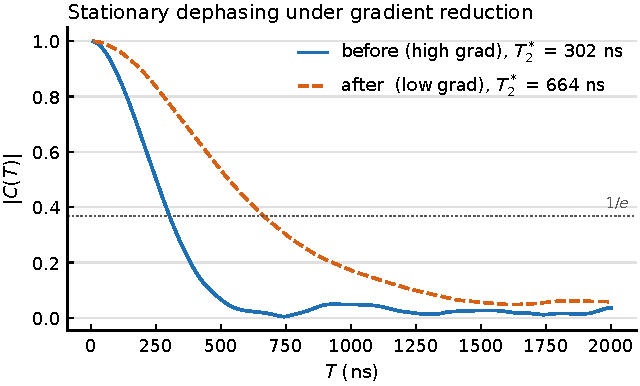
\includegraphics[width=0.7\columnwidth]{figures/gradient_halving.pdf}
\caption{Validation V1. Static-dot coherence decay $|C(T)|$ under
$1/f$ charge noise for a high and a halved magnetic gradient. Halving
the gradient increases $T_2^\ast$ from $302$ to $664$\,ns (ratio
$2.20$), within our $\pm20\%$ acceptance interval around the reported
ratio. Only the ratio is claimed; the
absolute values depend on the representative noise amplitude.}
\label{fig:v1}
\end{figure}

\subsection{Motional-narrowing trend (V2)}
For a periodic landscape with $1/f$ charge noise, the effective
$T_2^\ast$ improves as the shuttling velocity increases, from
$50$\,ns at $v=0$ to $3215$\,ns at $v=20$\,m/s (up to $64\times$),
reproducing the direction of the motional-narrowing improvement reported
in Ref.~\cite{krzywda_coherence_2026}; the $64\times$ magnitude is
specific to the present model and parameter set. This occurs
once the drive frequency $f_{\rm drive}=v/a$ moves above the dominant
noise band. The stationary baseline here is an effective static-gradient
model with the mean absolute periodic gradient
$\langle|B_{\rm long}'|\rangle\approx0.8$\,T/$\mu$m, so only the
\emph{relative} improvement is meaningful. \emph{Caveat:} we claim only
the direction of the trend; at very high velocity, orbital
non-adiabaticity (not modeled here) is expected to re-introduce error,
so unbounded improvement is not claimed.

\subsection{Filter-function suppression (V3)}
The periodic-shuttling filter function $F(f,T)$ suppresses
low-frequency ($f<1$\,MHz) sensitivity by about $2\times10^5$ relative
to a static dot. More directly, the actual dephasing functional, the
PSD-weighted overlap $\chi(T)=\int S_{\delta x}(f)F(f,T)\,df$, is
suppressed by about $5.8\times10^3$ ($T=1\,\mu$s, $v=10$\,m/s).
\emph{Caveat:} the filter-function shape and the realized dephasing
differ; a $10^5$-fold suppression of $F$ corresponds to only a
$10^3$-fold suppression of $\chi$, because dynamical decoupling lowers
the low-frequency response but introduces a sensitivity peak near
$f_{\rm drive}$ that overlaps the $1/f$ tail. Figure~\ref{fig:v3} shows
the filter function and the PSD-weighted integrand.

\begin{figure*}[t]
\centering
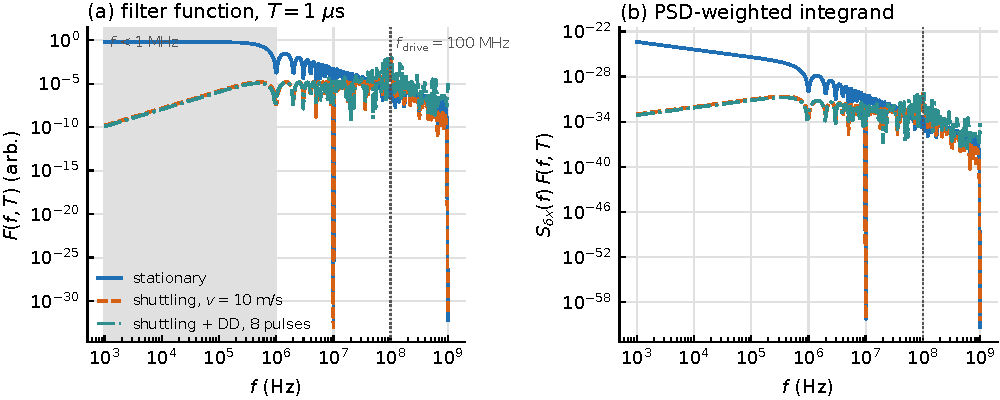
\includegraphics[width=0.92\textwidth]{figures/filter_suppression.pdf}
\caption{Validation V3. Left: the filter function $F(f,T)$ for a
static dot versus periodic shuttling (and shuttling with dynamical
decoupling), showing strong low-frequency ($f<1$\,MHz, shaded)
suppression. Right: the PSD-weighted integrand
$S_{\delta x}(f)\,F(f,T)$, whose integral is the realized dephasing;
its suppression ($\sim\!5.8\times10^3$) is smaller than that of $F$
alone ($\sim\!2\times10^5$) because decoupling introduces a
sensitivity feature near $f_{\rm drive}=v/a$.}
\label{fig:v3}
\end{figure*}

\subsection{Valley Landau--Zener dynamics (V4)}
The two-level valley time evolution reproduces the analytic
Landau--Zener diabatic probability
%
\begin{equation}
P_{\rm diab}=\exp\!\left(-\frac{2\pi\Delta_{v}^2}{\hbar\,|\dot \varepsilon_v|}\right)
\end{equation}
%
(where $\Delta_v$ is the valley avoided-crossing coupling and
$\varepsilon_v$ the diabatic valley detuning of the main text, distinct from
the physical valley splitting $E_{\rm VS}$; Fig.~\ref{fig:v4})
to within $0.28\%$ over a sweep-rate parameter range
$\gamma\in[0.1,10]$. In the adiabatic limit ($v\to0$) deep-pocket
traversal gives an excitation probability $P_e<10^{-5}$, and in the
diabatic limit ($v\ge30$\,m/s) the numerical and analytic predictions
agree to order of magnitude. \emph{Caveat:} this validates the
\emph{reduced} valley Landau--Zener physics of
Oda~\emph{et~al.}~\cite{oda_suppressing_2026}, not their full
optimized-protocol sequence; at
intermediate velocity ($1\le v\le10$\,m/s) St\"uckelberg interference
produces the expected order-of-magnitude departure from the single-event
formula, evidence that phase-coherent evolution between two crossings
is captured.

\begin{figure}[t]
\centering
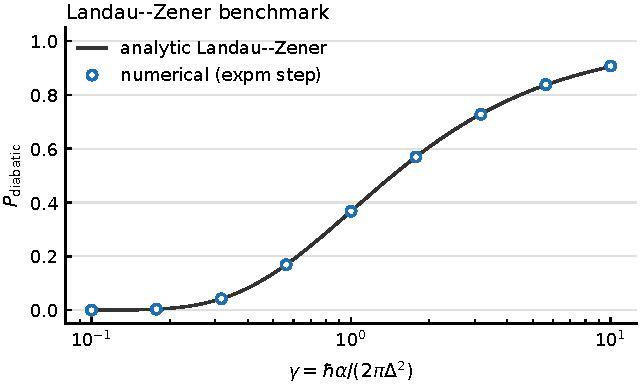
\includegraphics[width=0.7\columnwidth]{figures/landau_zener.pdf}
\caption{Validation V4. Diabatic transition probability after a linear
valley sweep, numerical (markers) versus the analytic Landau--Zener
formula (line), as a function of the sweep-rate parameter
$\gamma=\hbar\alpha/(2\pi\Delta_v^2)$. Agreement is within $0.28\%$
across the scanned range.}
\label{fig:v4}
\end{figure}

\subsection{Single-prism stray field (V5)}
The analytic stray field of a uniformly magnetized rectangular prism
(Engel-Herbert \& Hesjedal) is implemented in JAX and matches the
far-field dipole limit $B_z\to\mu_0 m/(2\pi d^3)$ to $0.06\%$:
$8.95\,\mu$T (numerical) versus $8.96\,\mu$T (dipole) on the $z$-axis at
$d=5\,\mu$m. Figure~\ref{fig:v5} shows the array field and its gradients
at two depths.

\begin{figure}[t]
\centering
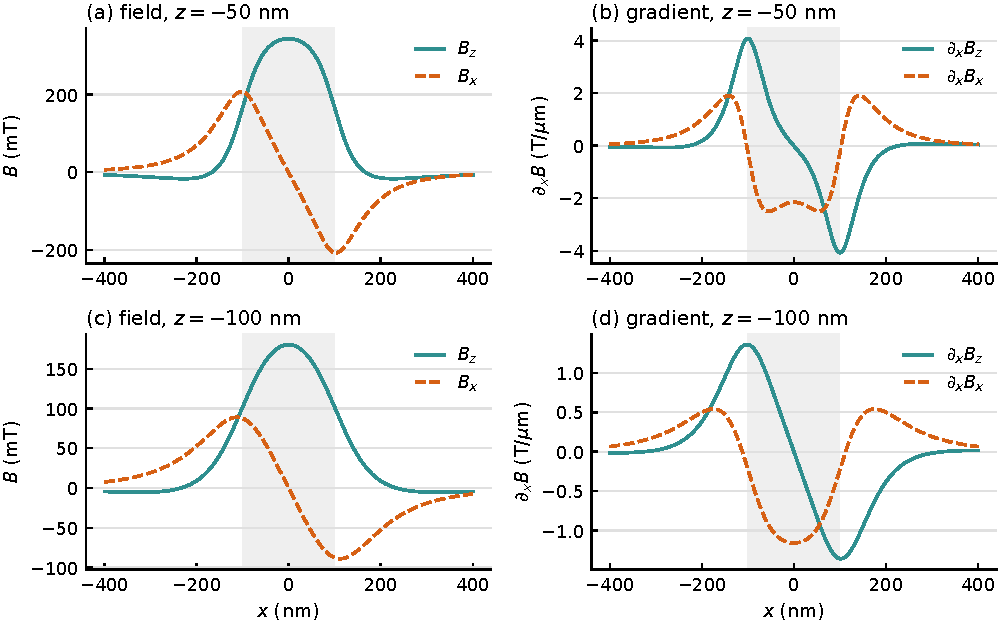
\includegraphics[width=0.95\columnwidth]{figures/prism_fields.pdf}
\caption{Validation V5/V6. Stray field $B_z,B_x$ (left) and their
position gradients via automatic differentiation (right) at two depths
below a micromagnet array. The gradient panels feed the coupling
profiles of the main text; the autodifferentiation underlying them is
validated against finite differences to $\le4\times10^{-6}$ (V6).}
\label{fig:v5}
\end{figure}

\subsection{Field- and gradient-scale consistency (V9)}
For a $50\times50\times30$\,nm magnet ($a=150$\,nm, depth $-50$\,nm) the
descriptor yields $\delta B_z=26.9$\,mT, peak gradient $1.19$\,mT/nm,
and mean gradient $0.72$\,mT/nm. These are comparable to the micromagnet
parameter scales $\delta B_z\sim5$--$30$\,mT and gradient
$\sim0.1$--$1$\,mT/nm used in the main text and reported for comparable
devices~\cite{yoneda_quantum-dot_2018,unseld_baseband_2025,langrock_blueprint_2023}:
$\delta B_z$ and the mean gradient fall inside those scales, and the peak
gradient sits just above the upper end. This check bears on the field and
gradient scales the chosen geometry produces, not on the magnet
dimensions themselves; the velocity range is motivated separately by
conveyor-mode shuttling studies.
\emph{Caveat:} a large magnet ($200\times200\times100$\,nm) gives
$\delta B_z\approx197$\,mT, about $10\times$ stronger; the main-text
baseline uses the small-magnet configuration, and the large-magnet case
is reserved as a strong-gradient stress test.
Table~\ref{tab:literature} summarizes the checks of this section.

\begin{table}[t]
\centering
\caption{Summary of literature and physical benchmark validations. Quantities
validated as ratios or trends are marked; absolute magnitudes that
depend on representative noise amplitudes are not claimed beyond the
stated sense.}
\label{tab:literature}
\begin{tabular}{llll}
\toprule
ID & quantity & reference / regime & result \\
\midrule
V1 & gradient-halving $T_2^\ast$ ratio & Krzywda~\cite{krzywda_coherence_2026}: reported $1.93$, our $\pm20\%$ band & $2.20$ (ratio) \\
V2 & motional-narrowing trend          & Krzywda~\cite{krzywda_coherence_2026}: direction only & up to $64\times$ \\
V3 & filter-function suppression       & static vs shuttling, this model & $F:2\times10^5$, $\chi:5.8\times10^3$ \\
V4 & valley Landau--Zener              & reduced Oda model~\cite{oda_suppressing_2026} & $<0.28\%$ \\
V5 & single-prism stray field          & dipole far-field limit       & $0.06\%$ \\
V9 & field/gradient scale              & device parameter scales      & comparable; peak gradient at upper end \\
\bottomrule
\end{tabular}
\end{table}

\section{Robustness of the response metrics}
\label{sec:robustness}
The main text's primary comparison is between cross-ansatz and cross-seed
disagreement in the nine-category thresholded label. This section examines three
robustness questions around it: whether the post-hoc ranking--classification
decoupling survives alternative ranked quantities, how much shared inactivity
contributes to the measured agreement, and how the label comparison behaves
when attention is restricted to comparisons with at least one two-channel
quadrant label.
Two candidate explanations are examined -- that the ranking and the classifier
simply weight the response channels differently, and that the comparison is
carried by conditions inactive in both members of a pair. Neither accounts for
the result.

\subsection{Channel weighting does not explain the decoupling}
The released magnitude $|\mathcal{R}|=\sqrt{\Delta P_v^2+\Delta\chi_\phi^2}$
weights the two channels equally in raw units, while the classifier judges each
channel against its own floor. Since $|\Delta\chi_\phi|$ is typically about a
decade larger than $|\Delta P_v|$, the raw-norm ranking is effectively
dominated by the dephasing channel, and this mismatch is the leading
alternative explanation of the decoupling reported in the main text.

Table~\ref{tab:weight} recomputes the pairwise rank correlations under
alternative ranked quantities. The diagnostic quantity is the gap between the
A/A$_{\rm pocket}$ and A/B$_z$ pairs, which differ by $33.3$ percentage points
in classification agreement at $n_{\rm real}=100$ ($35.9$ at $30$). If raw-unit
channel weighting were the main explanation, floor normalization should move
the ranking gap substantially toward the classification gap. It moves it only
from $0.003$ to $0.015$, and ranking each channel separately moves it less. Among the ranked quantities tested here, the one that tracks
classification agreement is the \emph{signed} dephasing response, whose gap
reaches $0.154$ and whose six-pair correlation with classification agreement is
$+0.880$. This implicates response-sign information as a leading contributor to
the decoupling.

Two limits on that reading. The six ansatz pairs are not independent --
A/A$_{\rm pocket}$ and A/B$_z$ share A -- so the six-pair correlations are
supporting evidence only, and the intermediate quantities change sign between
the two ensemble sizes. The classifier also uses floor crossing as well as
sign. The signed-$\Delta\chi_\phi$ result is a post-hoc diagnostic that
implicates sign information as a leading contributor; it is not a demonstrated
cause. Figure~\ref{fig:supp_robust}(a) shows the same comparison.

\begin{table}[t]
\centering
\caption{Pairwise rank correlation under alternative definitions of the ranked
quantity, and the resulting A/A$_{\rm pocket}$ against A/B$_z$ gap. The
classification-agreement gap for that pair of pairs is $0.359$ at
$n_{\rm real}=30$ and $0.333$ at $100$; a ranked quantity carrying the
explanation should close much of that distance. Six-pair ordering statistics are discussed in the
text and are not tabulated: only the released magnitude and the signed
$\Delta\chi_\phi$ are stable between the two ensemble sizes. Post-hoc
diagnostic.}
\label{tab:weight}
\small
\begin{tabular}{lcccc}
\toprule
 & \multicolumn{2}{c}{mean $\rho$} & \multicolumn{2}{c}{pair gap} \\
\cmidrule(lr){2-3}\cmidrule(lr){4-5}
ranked quantity & $n{=}30$ & $n{=}100$ & $n{=}30$ & $n{=}100$ \\
\midrule
released $|\mathcal{R}|$ & $0.914$ & $0.913$ & $0.0090$ & $0.0029$ \\
floor-normalized magnitude & $0.888$ & $0.896$ & $0.0197$ & $0.0146$ \\
$|\Delta P_v|$ only & $0.856$ & $0.869$ & $0.0010$ & $0.0100$ \\
$|\Delta\chi_\phi|$ only & $0.921$ & $0.917$ & $0.0002$ & $0.0049$ \\
$\Delta P_v$, signed & $0.846$ & $0.826$ & $0.0312$ & $0.0390$ \\
$\Delta\chi_\phi$, signed & $0.788$ & $0.765$ & $\mathbf{0.1299}$ & $\mathbf{0.1538}$ \\
\bottomrule
\end{tabular}
\end{table}

\subsection{Shared inactivity does not carry the contrast}
A shared \emph{below-threshold} assignment counts as agreement, so a large
inactive population could in principle manufacture both the agreement level and
the cross-ansatz versus cross-seed contrast. The main text reports the dilution
directly: at $n_{\rm real}=100$, $11$ of $108$ conditions are inactive under
every ansatz and block, and shared below-threshold assignments supply $44.6\%$
of ansatz-pair agreement and $44.9\%$ of seed-pair agreement.

As a pre-registered sensitivity analysis we recompute both estimands on the
subset of comparisons in which at least one member carries one of the four
two-channel quadrant labels. A comparison is excluded only when neither member
carries such a label; a single-channel or below-threshold assignment can still
appear as the other member of an included pair. The contrast survives and widens: cross-ansatz disagreement rises to
$0.523$ and cross-seed to $0.326$ at $n_{\rm real}=100$, a ratio of $1.61$
against $1.31$ unconditioned, and the union-conditioned cross-ansatz value stays
within $0.505$--$0.550$ across all eight registered checkpoints while the
cross-seed value falls from $0.656$ to $0.326$
[Fig.~\ref{fig:supp_robust}(b)]. Intersection conditioning is deliberately not
used: it would condition away the transitions the comparison measures.

\begin{figure}[t]
\centering
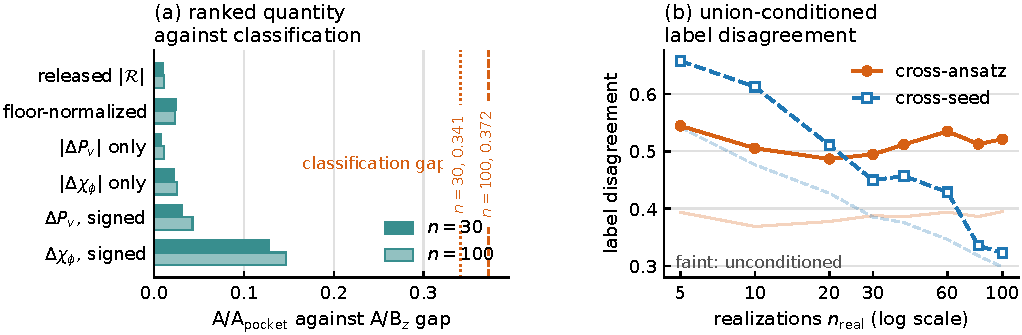
\includegraphics[width=\columnwidth]{figures/robustness_checks.pdf}
\caption{(a)~The A/A$_{\rm pocket}$ against A/B$_z$ gap under alternative
ranked quantities, at both endpoints; the dashed line is the corresponding
classification-agreement gap at $n_{\rm real}=100$ (dotted, at $30$). The
signed dephasing response comes closest among the tested quantities. (b)~Both estimands restricted to
comparisons in which at least one member carries a two-channel quadrant label,
across the eight registered checkpoints; faint lines are the unconditioned
estimands. The restriction widens the contrast.}
\label{fig:supp_robust}
\end{figure}

\subsection{Chance-corrected agreement}
Raw agreement can be inflated by skewed marginals, and \emph{below-threshold} is
the largest single category. Cohen's $\kappa$, computed on the same
nine-category label set, corrects for that. Table~\ref{tab:kappa} reports both
quantities at the two endpoints. No pair reaches strong agreement: $\kappa$ runs
from $0.345$ to $0.794$ at $n_{\rm real}=30$ and from $0.338$ to $0.777$ at
$100$, and the ordering is stable between them.

The two lowest values at both endpoints are A/A$_{\rm pocket}$ and
A$_{\rm pocket}$/B$_z$; both involve A$_{\rm pocket}$. The remaining
A$_{\rm pocket}$ pair, A$_{\rm pocket}$/B$_x$, lies in the middle group. The three pairs containing B$_x$ sit together in the middle, and A
versus B$_z$ -- the two profiles differing only by the hot-spot weighting -- is
highest, and still disagrees on about a fifth of conditions. Four profiles
cannot support a factorial attribution, so these are three specified diagnostic
contrasts and not an identification of which physical ingredient drives the
disagreement.

\begin{table}[t]
\centering
\caption{Pairwise classification agreement and chance-corrected Cohen's
$\kappa$ over the nine-category thresholded label, at the pre-registered
endpoint and the registered follow-up endpoint. Rows are ordered by agreement at
$n_{\rm real}=100$.}
\label{tab:kappa}
\small
\begin{tabular}{lcccc}
\toprule
 & \multicolumn{2}{c}{$n_{\rm real}=30$} & \multicolumn{2}{c}{$n_{\rm real}=100$} \\
\cmidrule(lr){2-3}\cmidrule(lr){4-5}
pair & agreement & $\kappa$ & agreement & $\kappa$ \\
\midrule
A vs A$_{\rm pocket}$         & $46.9\%$ & $0.345$ & $48.3\%$ & $0.338$ \\
A$_{\rm pocket}$ vs B$_z$     & $48.1\%$ & $0.358$ & $50.4\%$ & $0.365$ \\
A vs B$_x$                    & $61.3\%$ & $0.533$ & $60.7\%$ & $0.512$ \\
A$_{\rm pocket}$ vs B$_x$     & $60.9\%$ & $0.475$ & $60.7\%$ & $0.452$ \\
B$_z$ vs B$_x$                & $63.3\%$ & $0.557$ & $60.7\%$ & $0.513$ \\
A vs B$_z$                    & $82.8\%$ & $0.794$ & $81.7\%$ & $0.777$ \\
\bottomrule
\end{tabular}
\end{table}

The three pairs containing B$_x$ agree on exactly $328$ of $540$ comparisons at
$n_{\rm real}=100$. This is a coincidence of three near-equal counts, not a
structural identity: the same three values are $0.613$, $0.609$ and $0.633$ at
$n_{\rm real}=30$ and $0.600$, $0.607$ and $0.615$ at $5$.

\subsection{Absolute performance proxies (archival)}
The main text reports baseline-relative responses. For scale, Table~\ref{tab:abs}
lists the absolute full-model (M2) leakage $P_v^{\mathrm{M2}}$, dephasing
variance $\chi_\phi^{\mathrm{M2}}$, and the derived phase-error proxy
$p_\phi=(1-e^{-\chi_\phi/2})/2$, averaged over the baseline geometry, both
pocket cases, and $v\in\{5,10,20\}$\,m/s.

These archived runs occupy the numerical scales shown, spanning a factor of
$3.4$ in $P_v^{\mathrm{M2}}$ and a factor of $16$ in
$\chi_\phi^{\mathrm{M2}}$. The spread between ans\"atze cannot be attributed
to the ansatz: the values were computed under the earlier seeding scheme at
$n_{\rm real}=5$, so each ansatz saw a different noise realization. The table
is reported for scale only and supports no cross-ansatz conclusion.

\begin{table}[t]
\centering
\caption{Absolute full-model performance proxies per ansatz (baseline geometry,
both pocket cases $x_c=0$ and $x_c=25$\,nm, $v\in\{5,10,20\}$\,m/s,
$n_{\rm real}=5$, $1/f$ noise with $f_{\rm high}=10^7$\,Hz). Archival values
computed under the earlier seeding scheme; reported for scale only.}
\label{tab:abs}
\small
\begin{tabular}{lccc}
\toprule
ansatz & $P_v^{\mathrm{M2}}$ & $\chi_\phi^{\mathrm{M2}}$ & $p_\phi^{\mathrm{M2}}$ \\
\midrule
A                  & $0.259$ & $0.0195$ & $0.0049$ \\
A$_{\rm pocket}$   & $0.0786$ & $0.0106$ & $0.0026$ \\
B$_z$              & $0.266$ & $0.172$ & $0.0413$ \\
B$_x$              & $0.107$ & $0.0169$ & $0.0042$ \\
\bottomrule
\end{tabular}
\end{table}

\section{Relation to the main text}
The numerical-consistency checks (V0--V8) certify the field model, its
gradients, and the time-evolution engine that produce every quantity in
the main-text atlas. The literature and physical benchmark checks
(V1--V9) support the representative parameter values (Table~I of the main
text). V9 verifies that the controlled-reference geometry produces field
and gradient scales comparable to those of relevant micromagnet devices,
while the velocity sweep is motivated separately by conveyor-mode
shuttling studies. V1--V3 test the dephasing response to gradients, and
V4 tests the reduced valley dynamics. None of these checks
validates the spin--valley coupling profile $\lambda_{sv}(x)$ itself,
which the main text treats as a phenomenological diagnostic ansatz; the
sensitivity of the conclusions to that choice is the subject of the main text.
Section~\ref{sec:robustness} is separate from this suite: it does not validate
the simulator, but tests the robustness of the post-hoc ranking diagnostic and
the sensitivity of the primary label comparison to restricting attention to
comparisons with at least one two-channel quadrant label.

\clearpage
\bibliographystyle{aipnum4-2}
\bibliography{ref}

\end{document}
